\documentclass[conference]{IEEEtran}
\usepackage{graphicx}
\IEEEoverridecommandlockouts
% The preceding line is only needed to identify funding in the first footnote. If that is unneeded, please comment it out.
\usepackage{cite}
\usepackage{amsmath,amssymb,amsfonts}
\usepackage{algorithmic}
\usepackage{graphicx}
\usepackage{textcomp}
\usepackage{xcolor}
\def\BibTeX{{\rm B\kern-.05em{\sc i\kern-.025em b}\kern-.08em
    T\kern-.1667em\lower.7ex\hbox{E}\kern-.125emX}}
\renewcommand{\thesubsection}{\thesection.\alph{subsection}}
\begin{document}

\title{BareTag Tool-Tracker\\
{\footnotesize {Team 3 - University of Massachusetts Amherst Senior Design Project 2025 }}
}

\author{\IEEEauthorblockN{Walter Tebbetts}
\textit{CompE}\\
\textit{Software Lead}

\and
\IEEEauthorblockN{Sean Brown}
\textit{CompE}\\
\textit{Logistics Lead}

\and
\IEEEauthorblockN{Ken Su}
\textit{CompE}\\
\textit{Budget Lead}

\and
\IEEEauthorblockN{Connor McGarry}
\textit{CompE}\\
\textit{Hardware Lead}

}

\maketitle

\begin{abstract}
    Over the past 10 years, the majority of tools on a construction 
    site have converted from wired to battery-powered. While this 
    makes tools easy to move around, it also makes them easy to misplace
    and an easier target for theives. Data indicates that the construction
    idustry suffered nearly \$1,000,000,000 in loses due to tool theft in
    2016 alone [1], strongly indicating the need for a robust and effective 
    theft mitigation system. We propose the BareTag Tool Tracker, a novel
    approach to tool tracking that utilizes Ultra-Wideband(UWB) and Bluetooth 
    Low-Energy(BLE) radio in order to real-time track tools, materials, or other 
    valuable items on a construction site. The system utilizes a series
    of pre-placed Anchor posts, that send UWB pings to a Tag that is connected
    to a tool. Each Anchor can then calculate its distance to a Tag, relaying
    that information to a Base station over Long Range(LoRa) radio. The 
    base station runs the aggregated distance data through a multilateration
    algorithm that can calculate the Tag's location with $\pm$ 10 cm accuracy.
    The calculated location is then output to a local terminal, as well as 
    uploaded to a cloud database for future reference. Altogether, the BareTag Tool-Tracker
    is highly accurate ($\pm$ 10 cm), low-power (1 year of battery life), and
    scalable (increase range by adding additional Anchors).
\end{abstract}


\section{Introduction}
On constructions sites tools are constantly being misplaced causing workers to spend extra time searching and waiting before 
returning to their assignments. Furthermore, in recent years research has 
shown that theft on constructions sites has built up costs for construction 
companies and slowing down projects, very detrimental for small companies. 
Many different approaches have been taken to solve this 
growing issue. 

\subsection{Significance}

In 2016 it was estimated that in the United States alone \$1,000,000,000 
worth of construction tools were stolen [1]. A survey by the Charted 
Institute of Building discovered that out of the 1000 construction mangers 
interviewed, a third responded that they had experienced theft weekly on 
their sites. It was estimated that each of these weekly incidents cost the 
business an average of \$6,000, in some cases, in a single night the site 
had lost \$100,000 worth of equipment [2]. What’s worse is that this is a 
growing case. The FBI has reported that in 2021, theft on construction 
sites had outgrown theft in convenience stores [3]. Many managers have 
reported that these incidents have escalated to organized crime with 
evidence of sophisticated planning and coordinated executions. [2]. 
Theft on the site is not only costly to the business owners but also 
inconvenient for the construction workers and their managers. 
Due to the lack of proper tools construction workers may not continue with
their assignments and managers have to keep pushing deadlines. The 
result of this costs the business not just in extra wages, but also 
extra insurance and reputation [2]. 

\subsection{Context and Survey of Similar Solutions}

The general problem of item tracking has had many attempted solutions 
and continues to be a problem of interest today. In designing our system, 
we extensively researched many similar solutions to examine how these 
solutions fall short of achieving our system’s goals. Other solutions 
we have examined use various technology for tracking such as: AI image 
processing, GPS, Bluetooth, and Ultra-Wideband.

One comparable solution that utilizes image processing methods is offered 
by SIRIX. Their approach involves human and AI-assisted item tracking, 
using two types of cameras: wide-angle and thermal. These cameras are 
strategically placed throughout the job site and are monitored 24/7 by both
human operators and AI [4]. However, this solution is highly unreliable 
and unsustainable due to the presence of blind spots that fall outside 
the cameras' field of view, leaving certain areas unprotected. 
Additionally, human judgments and AI decision-making can introduce 
further response time, potentially allowing thieves to escape with 
stolen items before any alert is triggered. Another concerning issue 
is with the way that the system is powered. Attackers, especially a 
criminal organization as mentioned in the problem statement could easily 
disable the system by cutting the power generator or energy source, 
rendering it inoperative, leaving the remote surveillance team with no 
recourse other than calling the authorities. While both SIRIX and 
BareTag offer 24/7 security systems, only BareTag qualifies as a 
true round-the-clock security measure. BareTag does not depend on 
human or AI intervention to ensure tools and materials are secure. 
Additionally, BareTag's low power consumption allows it to operate 
more efficiently across diverse terrains, offering higher portability 
and flexibility compared to the energy-intensive SIRIX system.

Another comparable solution we evaluated is a commercial system called 
GoCodes, which specifically addresses the issue of tool tracking. This 
system employs continuous GPS tracking to monitor valuable equipment 
within a geofence, helping businesses prevent the loss or theft of tools. 
While it offers effective on-site tracking, off-site tracking relies on 
individuals scanning QR codes placed on the tools. If a user scans the 
QR code, the item's location outside of the geofence can be updated [5]. 
However, this approach has a significant flaw — no tool thief would 
voluntarily scan the QR code, and they could easily remove the codes 
from the tools, eliminating any trace of the theft. Although GoCodes 
provides a workable solution, it has several drawbacks that our system 
aims to overcome. For one, GPS tracking is power-intensive, often requiring
frequent battery replacements for the trackers. Additionally, GPS 
tracking needs an unobstructed line-of-sight to function efficiently, 
which can be compromised in dynamic construction environments. 
Furthermore, our system is designed to operate in very rural construction 
areas where satellite connectivity may be limited. Unlike GPS, which 
requires a strong satellite connection for accurate tracking, 
ultra-wideband (UWB) technology, which our system uses, does not rely on 
satellites, making it more reliable in such environments.

A common solution and a more reliable approach is using the Apple AirTags.
In the Apple AirTags, there are BLE modules that help it communicate 
with other iPhones to create the Find My network. Additionally, it has 
UWB modules that allow the user to get a more accurate location of where 
the tag is once the AirTag is close enough to the user’s iPhone [6]. This 
creates a well-rounded system to let users get a general idea of where 
their items are with a battery life of up to a year. The difference 
between the BareTag and the AirTag is that the BareTag is used for 
accurately tracking high-value items within the set UWB perimeter. 
BareTag emphasizes the use of the UWB module so construction workers 
can easily find their tools, along with an additional BLE module for 
the Find My Network feature outside of the set perimeter. Unlike Airtag, 
our system aims to not only track and retrieve items but also to accurately 
and reliability track tools to optimize efficiency.

The final solution takes a similar approach to BareTag. Pozyx tracks 
items indoors by installing UWB anchors throughout the building, which 
communicate with UWB tags. These anchors are height-adjustable and 
plugged into walls. Once configured and registered in the system, 
items can be geofenced, and the collected data can be used to optimize 
workflow and labor efficiency [7]. While Pozyx offers an effective 
indoor tracking solution, it is less efficient in outdoor environments. 
In locations like construction sites, where power availability may be 
limited, anchor placement becomes a significant challenge. Additionally, 
even though Pozyx’s UWB tags are advertised to have a battery life of over 
five years, they are bulky and lack a low-power option. In contrast, 
BareTag’s anchors come with pre-installed communication systems and 
built-in batteries, making the system more portable and scalable. 
Furthermore, BareTag’s tags feature a built-in accelerometer with an 
automatic sleep function to maximize power efficiency. This not only 
extends battery life but also reduces the frequency of battery 
replacements, saving time and resources. In summary, BareTag's anchors 
do not rely on external power sources, and the tags are equipped with a 
low-power solution, making them more suitable for outdoor and construction 
site use compared to Pozyx’s solution.

\subsection{Societal Impacts}

Our system can positively benefit all of society. As a tool tracking 
system made for construction workers, they are the most obvious group 
of people who benefit from this system. With construction workers being 
the primary users of our system, many of our design choices will be made 
specifically for the system to be easily used by the average construction 
worker. We want to create a user-interface that helps construction workers 
track their tools without having to do any additional work of their own. 
While this will greatly help construction workers find their tools and 
not have to worry about their tools being stolen, it benefits owners of 
construction firms even more. With accurate tool tracking, they can 
ensure their workers are working as efficiently as possible and not 
wasting their time looking around sites for tools. Owners of construction 
companies are also the ones responsible for supplying their workers with 
the tools needed to complete jobs. We want our system to reduce these 
costs for construction firm owners by reducing the loss and theft of 
their very expensive tools. Preventing theft and increasing the 
efficiency of workers can help a construction firm look more professional 
and hireable by employers that need construction work done. Our system 
aims to help construction teams work quicker to efficiently finish jobs 
which will increase the number of jobs they can take. Because our system 
increases construction efficiency, anyone benefiting from the construction 
of literally anything can benefit from it as well. The only people that 
will be hurt by our system are thieves that will be caught stealing 
expensive tools by our system.

\subsection{Goals, Specifications and Testing Plan}

The BareTag Tool Tracker will implement the following goals, 1. Real-time 
tracking within a specified zone, 2. Precise accuracy for tracking within 
the zone, 3. Low Power,  4. Reliability outside the zone, 5. Scalability.

The specifications listed in Table 1 demonstrate the goals that our project 
aims to achieve by the time that we have a finalized product.
\begin{center}
\begin{table}
\caption{Design Goals and Testing Plan}
\begin{tabular}{|p{4cm}|p{4cm}|}
    \hline
    \textbf{Specification}  & \textbf{Testing Plan}\\
    \hline
    The system will track an item’s geo-coordinates with a reliability of 
    95\% within a specified 100 m x 100 m zone. 
    &
    Ping the Tag at randomized coordinates within the Sustainable 
    Engineering construction site.\\
    \hline
    The system will have less than 50 cm precision for tracking within 
    the specified zone.
    &
    Compare Tag’s measured location to its actual location 
    within a predefined grid.\\
    \hline
    The system will operate 24/7 for ~1 year without 
    replacing the batteries.
    &
    Measure the power consumption of the system in multiple modes.\\
    \hline
    Ensure that the Tag can be tracked via the Find My network outside 
    of the UWB zone.
    &
    Confirm tracking accuracy in scenarios with different saturations 
    of Find My devices by comparing with AirTags in the same location.\\
    \hline
    Should easily be scalable to increase the range of the UWB perimeter 
    by adding more Anchors at desired locations.
    &
    Demonstrate that a Tag’s trackable range in the UWB zone increases 
    when adding a new Anchor.\\
    \hline
\end{tabular}
\end{table}
\end{center}


\section{DESIGN}

This section describes the system design including design alternatives, 
design justifications, and hardware and software block diagrams.

\subsection{Overview}
At a high level, the BareTag Tool Tracker utilizes Ultra-Wideband (UWB) and 
Bluetooth Low Energy (BLE) radio in order to real-time track an 
item's location on a construction site. The technology at the core of our 
design is UWB radio. UWB radio is a form of radio communication that 
utilizes pulses of radio energy at specifically timed intervals in order 
to transmit information. This protocol is not ideal for data communication, 
but is very accurate in performing distance ranging. With two UWB 
transceivers, one configured as the controller (Anchor) and the other 
configured as the responder (Tag), the Anchor can range it's distance
to the Tag via UWB pings. The Anchor begins by sending a ping with 
the desired Tag's ID encoded, the Tag will almost immediately send 
back a response ping, the Anchor can then use the time between when it 
sent its ping to when it received the Tag's ping, in order to 
calculate the distance between the two transceivers. 

\[ d = \frac{\frac{ToF}{2}}{c} \]

Where $d$ is distance between the Anchor and Tag, 
$ToF$ is time of flight, and $c$ is the speed of light.

With distance measurements between 3 Anchors and 1 Tag, we
can preform a trilateration algorithm in order to calculate
the Tag's location within our site.

The equations for the three circles (Anchor to Tag distance):

\[(x - x_1)^2 + (y - y_1)^2 = r_1^2\]
\[(x - x_2)^2 + (y - y_2)^2 = r_2^2\]
\[(x - x_3)^2 + (y - y_3)^2 = r_3^2\]

Where $r_i$ is the distance from an Anchor to a Tag, $(x_i, y_i)$ are 
the cordinates for each Anchor on a 2D $x,y$ plane, and $(x,y)$ are the coordinates
for the Tag we are trying to locate.\\
Next we subtract the second equation from the first:

\[(-2x_1 + 2x_2)x + (-2y_1 + 2y_2)y = r_1^2 - r_2^2 - x_1^2 + x_2^2 - y_1^2 + y_2^2\]

Likewise, subtract the third equation from the second:
\[(-2x_2 + 2x_3)x + (-2y_2 + 2y_3)y = r_2^2 - r_3^2 - x_2^2 + x_3^2 - y_2^2 + y_3^2\]

Re-writing these two equations using A, B, C, D, E, and F:
\[Ax + By = C\]
\[Dx + Ey = F\]

Finally, the Tag's $(x,y)$ coordinates are:
\[x = \frac{CE - FB}{EA - BD}\]
\[y = \frac{CD - AF}{BD - AE}\]

Once the Tag's location has been calculated via our trilateration algorithm,
the Tag's location will be output to a local terminal, as well as 
uploaded to a cloud database. Outputting to a local terminal allows us to
have the system function without the need for an internet connection, 
something that may not be available on rural construction sites. If internet
is available, we can upload location to cloud database. With location data
stored remotely, any user with internet access can get their Tag's current
location, or past location.

Aditionally, as one of our main goals is to prevent theft, when a Tag
leaves the designated construction site, a notification will be sent to 
the user, letting them know that one of their Tag's has left the site.
To continue to track the Tag once it leaves the construction site, we will
turn off the Tag's UWB radio, and turn on the Tag's BLE radio. Using BLE
advertisements, the Tag will be able to communicate with nearby devices that
are using the Apple Find My protocol. The Find My protocol allows BLE devices
to be tracked with around 10 meter accuracy when in loactions saturated with 
Apple devices. With this tracking outside of the construction site, users 
can not only keep track of their tools on a construction site, but also track
down stolen tools outside of the construction site. To help integrate our
Tags into the Find My network, we will be using the open source project,
openhaystack. 

Openhaystack, is an open source project originating from TU Darmstadt, that
utilizes Find My's open API, as well as a collection of reverse engineering
and security analysis work to allow generic BLE devices to be tracked via
Apple's Find My network.

Altogether, the BareTag Tool Tracker utilizes UWB and BLE in order to real
time track the location of Tags on and off a construction site. The design
combines existing solutions for item tracking with UWB as well as the robust
and expansive Find My network to prevent tool theft and increase construction
site efficiency.  

\begin{figure}
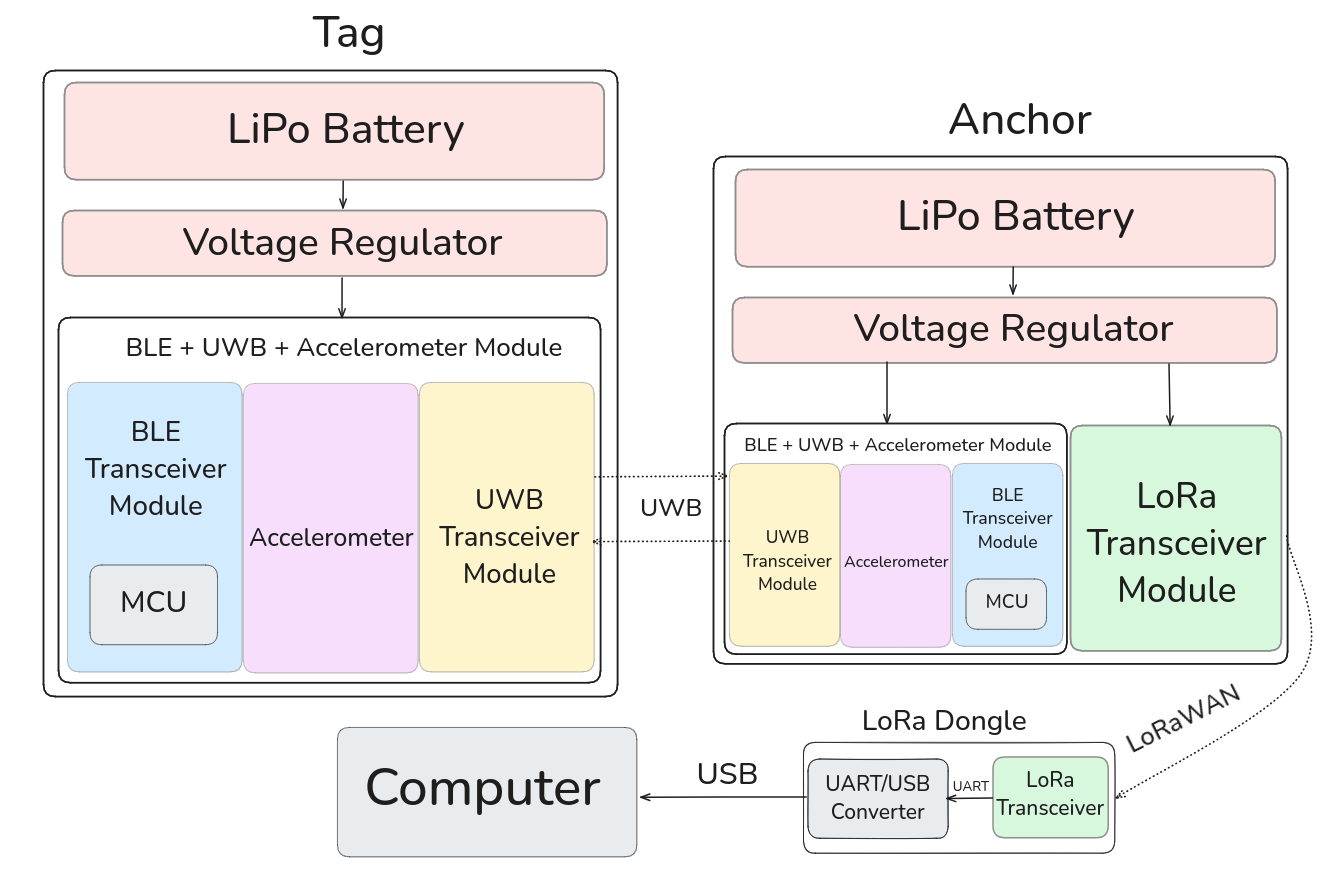
\includegraphics[scale=0.185]{Screenshot from 2024-10-18 21-37-02.png}
\caption{Full system hardware block diagram}
\end{figure}

\subsection{Tag}\label{AA}
The Tag refers to the trackable device that will be attached to the tools 
on a worksite. The goal is for the Tags to be less than 31.9mm2, which is 
of a similar size to the Apple Airtag. The thickness of the Tags is aimed 
to be under 16mm, with the primary contributor to this size being the 
pouch cell 290mAh Lithium Polymer battery. The peak current draw of the 
Tag is 45mA and is out of the range that a coin cell could support, 
which led to the decision to use a LiPo that fits within our area size 
goals at 25 mm x 28mm. We are aiming for a one year battery life.
The primary part of the Tag is the Qorvo DWM3001C. This module is driven 
by the nRF52833 MCU, and includes BLE, UWB, and accelerometer 
functionality. The DWM3001 provides UWB functionality and has an 
integrated PCB antenna which requires a keep-out zone in the Tag. 
BLE is provided by the nRF52833. This MCU is built on an ARM Cortex 
M4 and operates in the 2.4GHz band. This MCU is programmable over 
JTAG and thus requires a JTAG interface to be added to the Tag PCBs. 
The accelerometer is the LIS12DH, and is used to wake up the module 
upon motion detection. The module will set the interrupt pin on the 
DWM3001 high when there is motion detected. Otherwise, the Tag is in a 
low power mode to save battery life and is not receiving UWB pings. 
Therefore, before the tag goes to sleep the location needs to be checked 
to determine the resting location. The Tag has the BLE radio turned off 
until it exits the UWB perimeter, at which point an interrupt pin turns 
it on to integrate into the Apple Find My network. At this point, the 
UWB module turns off to conserve power. The accelerometer still regulates 
the power mode of the Tag depending on motion to conserve power. This 
device draws a lot of concepts from ECE 523 and ECE 304, both of which 
have a heavy focus on minimizing power consumption via software and 
component selection. The TPS79933 voltage regulator has an output of 
3.3V when the input voltage is over 3.475V. This component is used in 
both the Tags and Anchors as both devices operate on a 3.7V input battery 
with 3.3V ideal operating voltage. 


\subsection{Anchor}
There needs to exist at least 3 anchors for the coordinates to be 
transmitted to the user. This is performed through multilateration. 
The Anchors use the same Qorvo DWM3001C modules as on the Tags as all 
of the submodules have a use case here too. The Anchors use UWB to ping 
the Tag and determine its location within the area defined by the 
proximity of the other anchors. They operate on this data using the 
nRF52833 MCU and send it to a host device over LoRaWAN. The RYLR998 
LoRa module in the Anchors operates within the required range for 
LoRaWAN of 902.3 to 914.9 MHz. This module communicates with the MCU 
via UART. The use of these LoRa modules means that the Host Device does 
not need to be exactly on the site of the construction due to the 
kilometers of range that LoRa supports. We will build the LoRaWAN 
protocol on top of LoRa using the nRF52833 MCU. The use of this MCU 
also means that we can take advantage of the BLE it provides and use 
it for a variety of functions. The GPS coordinates of the Anchors must 
be known in order to get the real-world position of the Tags. We can 
also use BLE to communicate with an anchor to alert that a Tag that is 
in BLE mode has been returned to the UWB-supported area. These features 
result in  more power consumption than the Tags, so a 2.2Ah Lithium Ion 
battery is used. This is possible due to less size constraints for the 
Anchors than of the Tag. The size of the Anchor is not a specification 
that matters, however they will be able to be mounted on posts or stuck 
in different site locations depending on the desired use and area to cover.
As stated before, the TPS79933 voltage regulator outputs 3.3V, which is 
the ideal operating voltage for the DWM3001C, along with the LoRa module. 


\subsection{Lora Dongle}
This device is a RYLR998 operating over a USB - UART connection with the 
Host Device. It allows for the Host Device to receive the Tag coordinate 
data and operate on it. The size of this device should account for the 
LoRa module plus a USB/UART converter (CP2102N). The size should be similar 
to that of a USB hub, as to not be an inconvenience to have attached to a 
small host device. As such, the dimensions should be approximately 32 x 18 
x 8 mm based on a combination of the component dimensions. 
The Dongle receives power from the CP2102N over a wired USB-C connection, 
so there is no need for an external power supply. 


\subsection{Host Device}

This device can be whatever system a supervisor desires to use as long as 
it can support a physical USB/Serial connection, or do so using adapters. 
The Host Device is backhauling the location data of each Tag to a database 
where the history of the tag locations can be mapped out to determine the 
daily path. This information is also displayed in real time on a map of 
the desired area. The Host Device is also running the macless-haystack 
Find My server, which acts as a means for tracking the Tags that have 
left the UWB area and are now using BLE to integrate with the Apple Find 
My network. The tags all have unique IDs that can be linked to tools or 
equipment, making it easy to parse the data and determine what items have 
been in what location. 


\begin{thebibliography}{00}
\bibitem{b1} ``2016 equipment theft report,'' 2016. [Online]. Available: https://www.ner.net/wp-content/uploads/2017/10/Annual-Theft-Report-2016.pdf. Accessed Oct. 19, 2024.
\bibitem{b2} ``Crime in the construction industry,'' 2013. [Online]. Available: https://www.ciob.org/sites/default/files/. Accessed Oct. 19, 2024.
\bibitem{b3} ``An exploratory look at thefts from construction sites,'' 2019. [Online]. http://ascpro0.ascweb.org/archives/cd/2019/paper/CPRT247002019.pdf. Accessed Oct. 19, 2024.
\bibitem{b4} ``Remote Video Monitoring,'' SirixMonitoring, Sep. 13, 2024. [Online]. Available: https://sirixmonitoring.com/remote-video-monitoring/. Accessed Oct. 04, 2024.
\bibitem{b5} ``Pros and Cons of Construction Equipment Tracking,'' Tool Tracking Software, Aug. 02, 2023. [Online]. Available:  https://gocodes.com/equipment-tracking-pros-cons/. Accessed: Oct. 04, 2024.
\bibitem{b6} ``Airtag VS GPS tracker, what is the difference ?,'' Beepings.com, 2021. [Online]. Available:https://beepings.com/airtag-vs-tracker/. Accessed: Oct. 04, 2024.
\bibitem{b7} ``Pozyx UWB Tags - Accurate ultra-wideband trackers,'' Pozyx.io, 2024. [Online]. Available: https://www.pozyx.io/products/hardware/. Accessed: Oct. 04. 2024.
\end{thebibliography}
\vspace{12pt}

\section*{Appendix}
\setcounter{subsection}{0}
\subsection{Design Alternatives}
Before settling on our current design, we considered many alternatives. 
In order to make our user-interface have real world terrain displayed 
while tracking our tags, we need to find the coordinate positions of our 
anchors. In order to do this, we originally considered putting GPS modules 
on our anchors, but decided instead on creating a mobile app that can be 
used to find the GPS of your phone when setting up the anchors. We decided 
on this in order to save money, as individual GPS modules range from 
\$20-\$40. We also considered purchasing a separate MCU, LoRa, and UWB 
module to design our anchor PCBs. We found this design too complex and 
instead decided on the same module as we are using in the Tags. We decided 
on this current design because we want the tags and anchors to have the 
same technology to be able to program them with the same libraries in 
order expedite software development. Batteries have been a prominent 
part of our design that we have put a lot of effort into deciding on. 
Because we want the Tags to be small enough to go inside of tools without 
manufacturers having to add room for them, we decided on very small 
batteries inside the tag. We also considered doing energy harvesting 
for the anchors to increase the battery life of them, but have decided 
on large batteries for the anchors because they are less size constrained 
compared to the Tags. In our original plan, we were going to backhaul our 
data to a cloud database in order for processing. After some consideration, 
we decided on sending the data to a self-hosted database to have increased 
control over the hardware, software, and configurations, which allows us to 
customize our database to meet our project’s needs. Having our own 
self-hosted database can also allow us to implement our own security 
measures, will be less expensive, and will have greater performance 
optimized for our specific workload.

\end{document}
